\documentclass[a4paper,12pt]{article}
\usepackage[12pt]{extsizes}




\usepackage{cmap}					% поиск в PDF
\usepackage{mathtext} 				% русские буквы в формулах
\usepackage[T2A]{fontenc}			% кодировка
\usepackage[utf8]{inputenc}			% кодировка исходного текста
\usepackage[english,russian]{babel}	% локализация и переносы
\usepackage{ulem}                   % зачеркнутый текст
\usepackage{amssymb}			% пакет математики
\usepackage{float}
\usepackage{amsmath}
\usepackage{graphicx}
\DeclareGraphicsExtensions{.png}

%%% Страница
%\usepackage{extsizes} % Возможность сделать 14-й шрифт
\usepackage[left=1cm,right=1cm,top=1cm,bottom=1cm]{geometry} % Простой способ задавать поля
\pagestyle{empty}

\begin{document}


\begin{center}
ФЕДЕРАЛЬНОЕ ГОСУДАРСТВЕННОЕ ОБРАЗОВАТЕЛЬНОЕ БЮДЖЕТНОЕ УЧРЕЖДЕНИЕ ВЫСШЕГО ОБРАЗОВАНИЯ

    \textbf{«ФИНАНСОВЫЙ УНИВЕРСИТЕТ ПРИ ПРАВИТЕЛЬСТВЕ РОССИЙСКОЙ ФЕДЕРАЦИИ»}

Факультет информационных технологий и анализа больших данных

Департамент анализа данных и машинного обучения

\textit{
	\textbf{Дисциплина: «Теория вероятностей и математическая статистика»}}

\textit{Направление подготовки: 01.03.02 «Прикладная математика и информатика»}

\textit{Профиль: «Анализ данных и принятие решений в экономике и финансах»}

\textit{Форма обучения очная, учебный 2020/2021 год, 4 семестр}

\textbf{Билет 119}

\end{center}

\begin{enumerate}


\item

Дайте определение случайной величины, которая имеет гамма-распределение $\Gamma(\alpha,  \lambda)$, и выведите основные свойства гамма-расределения. Запишите формулы для математичсекого ожидания
$\mathbb{E}(X)$ и дисперсии $\mathbb{V}ar(X)$ гамма-распределения


\item



Случайные величины $X$ и $Y$ независимы и имеют равномерное
распределение на отрезках $[0;10]$ и $[0;9]$ соответственно. Для случайной величины $Z=\frac{Y}{X}$ найдите: 
1) функцию распределения $F_Z(x)$;
2) плотность распределения $f_Z(x)$ и постройте график плотности;
3) вероятность $\P(0,\!719\leqslant Z\leqslant 1,\!005)$.


\item


(10) Известно, что доля возвратов по кредитам в банке имеет распределение $F(x) = x ^{\beta}, 0 \leqslant x \leqslant 1$.
Наблюдения показали, что в среднем она составляет $93,3333\%$. Методом моментов оцените параметр $\beta$ и
вероятность того, что она опуститься ниже $19\%$


\item

    
    Создайте эмперические совокупности  $\mathtt{\text{exp}}$ и $\mathtt{\text{sin}}$ вида $\mathtt{\text{exp}}(1),\mathtt{\text{exp}}(2), ..., \mathtt{\text{exp}}(85) $ и $\mathtt{\text{sin}}(1),\mathtt{\text{sin}}(2), ..., \mathtt{\text{sin}}(85). $

    Найдите эмпирическое среднее и эмпирическое стандартное отклонение совокупности $\mathtt{\text{exp}}$, её четвёртый эмпирический центральный момент и эмпирический эксцесс.

    Кроме того, найдите эмпирический коэффициент корреляции признаков $\mathtt{\text{exp}}$ и $\mathtt{\text{sin}}$ на совокупности натуральных чисел от $1$ до $85$.
    

\item


(10) Эмпирическое распределение признаков $X$ и $Y$ на генеральной совокупности $\Omega$ задано таблицей частот  
 
\begin{tabular}{ | c | c | c | c | }
\hline
 & $Y = 2$ & $Y = 4$ & $Y = 5$  \\ \hline
$X = 200$ & $28$ & $23$ & $3$\\ \hline
$X = 300$ & $2$ & $12$ & $32$\\
\hline
\end{tabular}

Из $\Omega$ случайным образом без возвращения извлекаются $5$ элементов. 
Пусть $\bar X$ и $\bar Y$ – средние значения признаков на выбранных элементах. 
Требуется найти: 1) математическое ожидание $\mathbb{E}(\bar Y)$; 2) стандартное отклонение $\sigma(\bar X)$ ; 
3) ковариацию $Cov(\bar X, \bar Y)$


\item


(10) Пусть $X _{1}$, $X _{2}$, $X _{3}$, $X _{4}$ выборка из $N(\theta, \sigma ^{2})$. Рассмотрим две оценки параметра $\theta$:
\[\hat \theta _{1} = \frac{2X _{1} + 3X _{2} + 4X _{3} + X _{4}}{10}, \hat \theta _{1} = \frac{2X _{1} + 3X _{2} + 2X _{3} + 3X _{4}}{10}\]
a) Покажите, что обе оценки несмещенные.
б) Какая из оценок оптимальная?


\end{enumerate}

\begin{figure}[H]
	Подготовил
	\hfill
	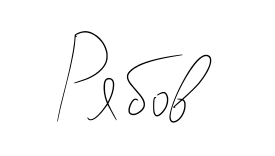
\includegraphics[width=2cm]{Prepared}
	П.Е. Рябов
\end{figure}


\begin{figure}[H]
	Утверждаю:\\
	Первый заместитель\\
	руководителя департамента\\
	Дата 01.06.2021
	\hfill
	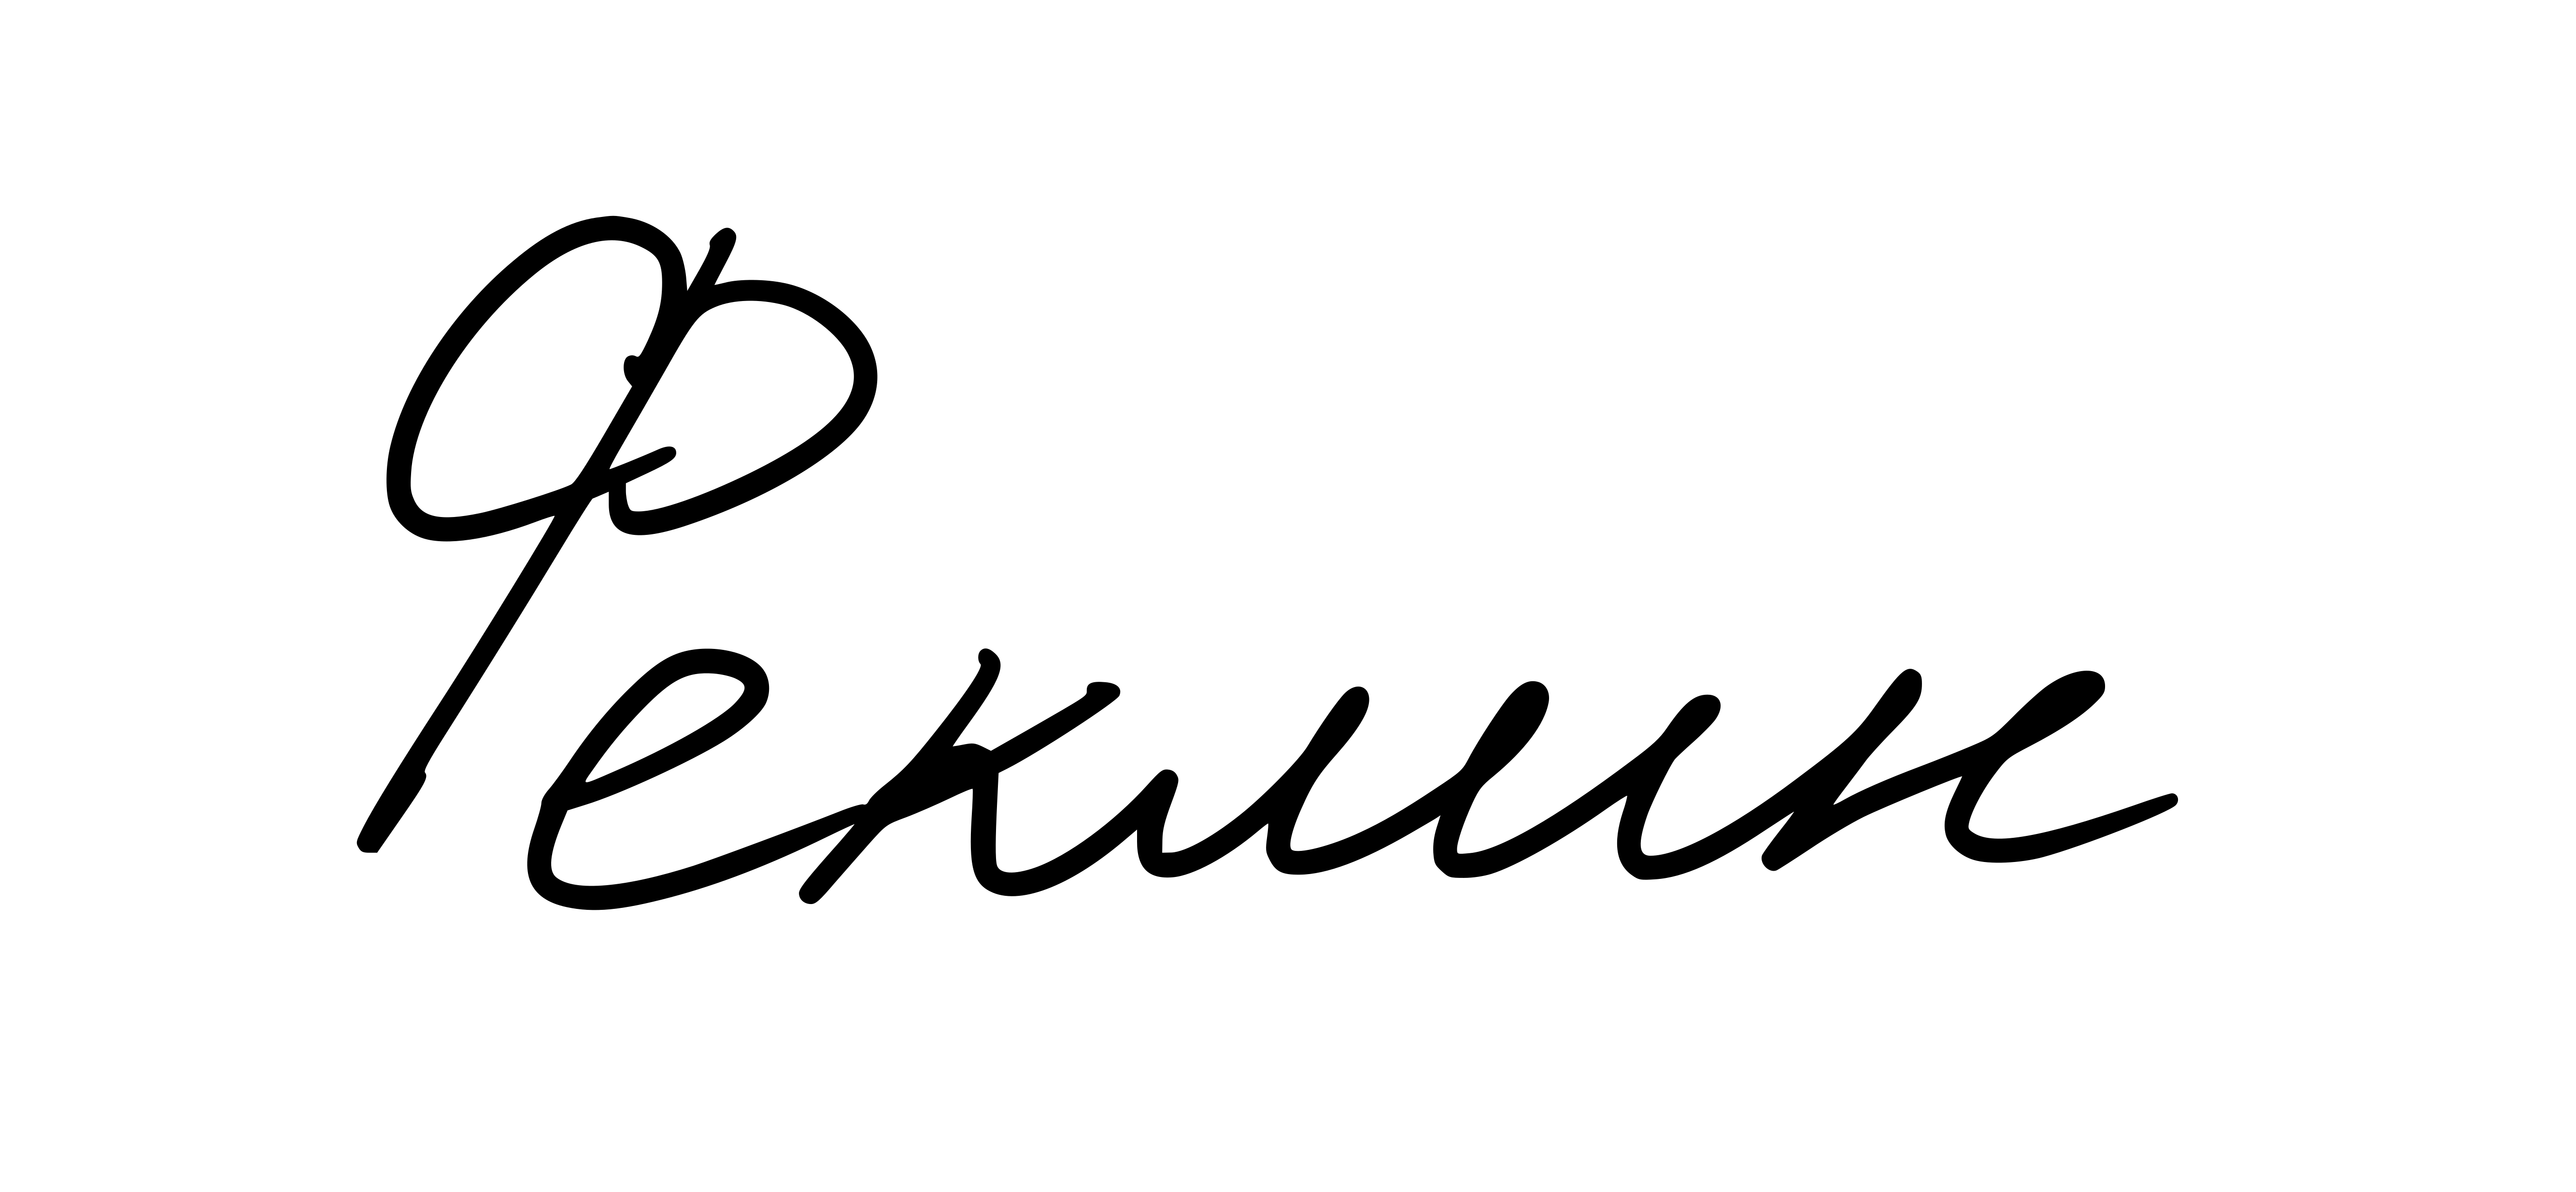
\includegraphics[width=2cm]{Approved}
	Феклин В.Г.
\end{figure}

\end{document}

